\documentclass{beamer}
\usepackage{graphicx}
\usepackage{listings}
%Information to be included in the title page:
  \title{850 Beamer Presentation}
\author{Wyatt McLeod}
\date{November 29, 2021}

\begin{document}

\frame{\titlepage}

\begin{frame}
\frametitle{Who Am I?}
Hello! My name is Wyatt McLeod. Here are some brief points about who I am:
  \begin{itemize}
\item I was born in Needles, CA on March 20th 1998.
\item I moved to Lincoln when I was 8 years old.
\item I went to Lincoln Northeast High School and just recently graduated from Augustana University in Sioux Falls, SD.
\item I am in the UNL Statistics PhD program.
\end{itemize}
\end{frame}

\begin{frame}{My Favorite Animal}
This is a picture of my favorite animal, the Shoebill Stork. This thing is just strange.

\begin{center}
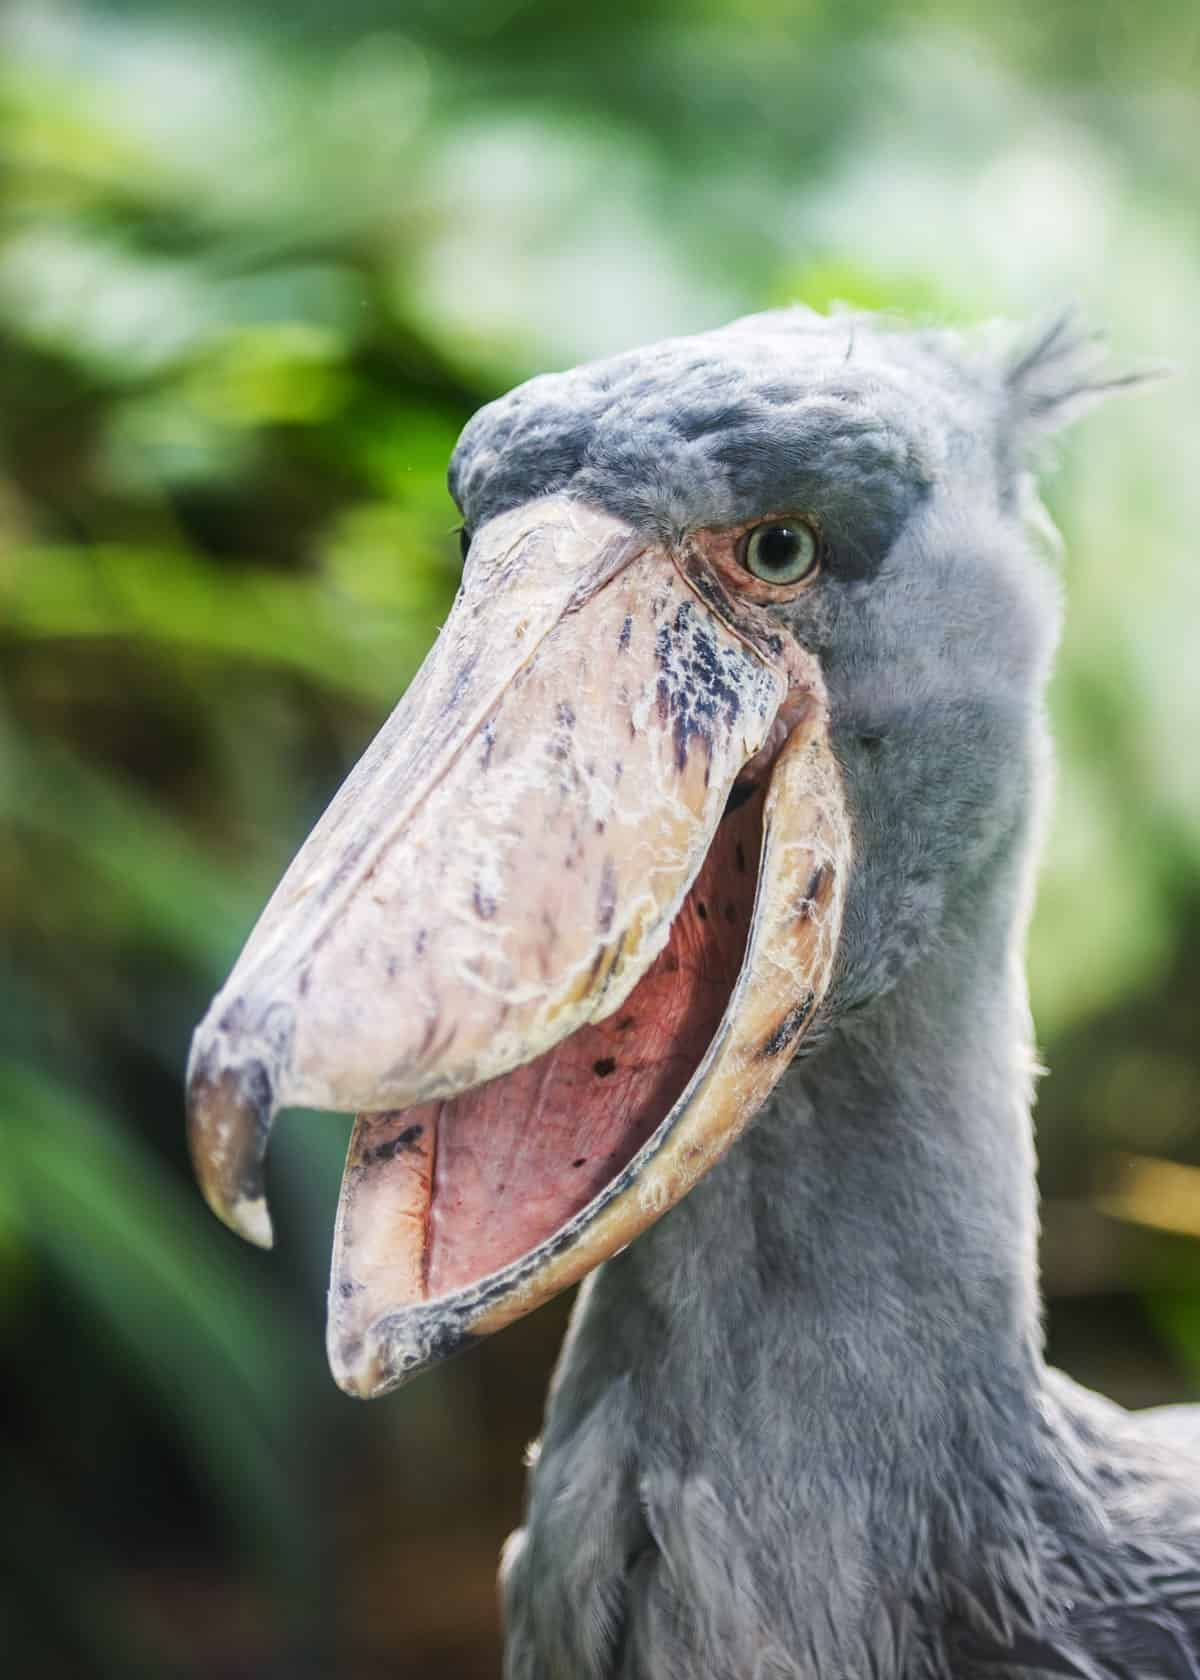
\includegraphics[scale=0.1]{shoebill-stork.jpg}
\end{center}
\end{frame}

\begin{frame}{My favorite plot from 850}
This is my favorite plot that I made in 850. It's my favorite because it was fun to make, and is super ugly.

<<graph,>>=
library(palmerpenguins)
library(ggplot2)

ggplot(data=penguins, aes(x = island, color = sex)) +
  geom_bar(position='dodge2', fill='light pink') + labs(title='Sex Count by Island', x='Island', y='Sex Count') + theme(
    panel.background = element_rect(fill='light pink'),
    panel.grid.major = element_line(color='black'),
    panel.grid.minor = element_line(color='light blue'),
    plot.background = element_rect(fill = 'light blue'),
    legend.position= 'bottom',
  ) + scale_color_manual(breaks=c('female', 'male', 'NA'), values=c('light blue', 'light grey', 'grey'))
@
\end{frame}

\begin{frame}{My Resume}
*if my slides worked, here is where the resume would go*
\end{frame}

\end{document}
